\section{Simulation}

\subsection{Animatlab}

Animatlab is a simulation environment that combines a physics engine with a
neuron simulation tool. It is very helpful for integrating physical systems
and sensor information easily into a synthetic nervous system.

The design tools for defining and testing a nervous system were also intrumental
to the success of the new controller design.

\subsection{Python Numerical Simulation}

During the development of the original controller design, an additional
simulation environment was created in Python. Due to the complicated nature of
the controller design, it was infeasible to prove the stability and other
properties of the controller directly, especially with changing internal
parameters. Instead, the Python simulation environment was used to gradually add
in expected physical effects to see how the algorithm behaved.

The pneumatic actuators and their existing pressure controller were simulated 
at varying degrees of fidelity. Originally, a simple model of the actuators
was used that emulated their non-linear behavior for applying torque, but didn't
include damping effects, load or limitations of the underlying pressure
controller. Over time these effects were added in until a high fidelity model of
a joint was controlled with the algorithm. This simulation environment also
enabled the testing and verification of a simplified internal model for
replication within the neuron controller. Without the Python simulation
environment, this evidence-based design of models would not have been as easy to
iterate.

\section{Testing and Verification}

One of the key steps for verifying the neuron controller was a series of tests
using the DataTool functionality of Animatlab. By simulating inputs to subsets
of the network, the output can be verified against the Python controller
implementation or other pre-computed values. This independent testing further
reinforces the value of the functional sub-network approach.

\subsection{Neurons}

One of the most important aspects of the functional subnetwork approach is that
individual subnetworks can be tuned, verified and then combined with the larger
network. In order to better tune individual networks, a testing rig was set up
within the larger network to allow for subnetwork verification. The typical
interface neurons are disabled and special test driver neurons (highlighted in
yellow) are enabled. This allows for the driving of custom input signals and
combinations of signals in order to verify the output value and speed. 
See \myref{fig:TestNetworkT2P} for a good example.

\begin{figure}
\centering
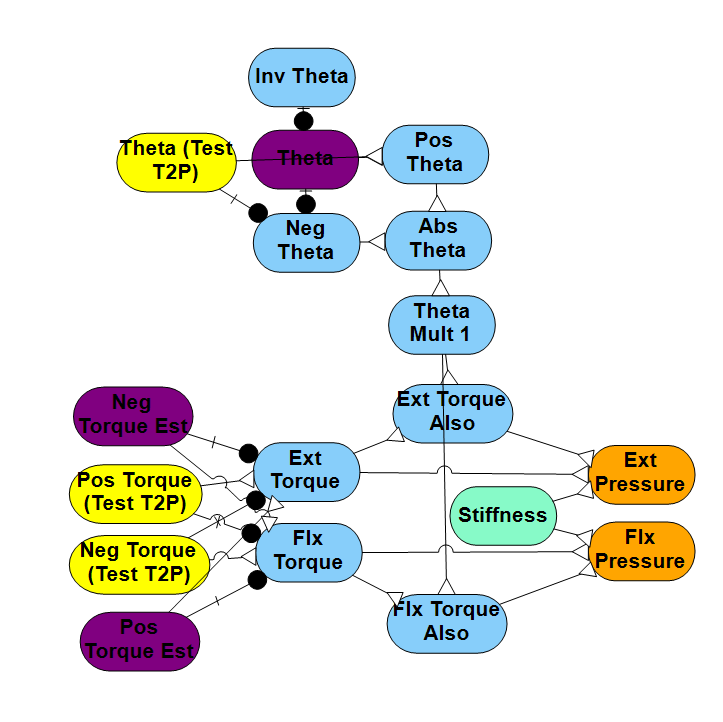
\includegraphics[height=3.5in]{methods/TestVisualT2P}
\caption{Torque to Pressure network with test and actual inputs shown}
\label{fig:TestNetworkT2P}
\end{figure}

This particular network is designed to convert a desired torque from the rest
of the network to the pressure for the extension and flexion pneumatic actuators.
With this network, the input neurons (in purple)
are disabled for testing and the test neurons are enabled. From there, inputs
are driven, as seen in \myref{fig:TestNetworkInputs}. This allows the inputs to 
be mapped to real world values, the real world inputs to be mapped to outputs, 
and the real world outputs to be mapped back to neuron voltages. Through this
a test framework is built where the output can be visually compared to the 
reference to ensure neuron networks are working as intended. See 
\myref{chap:results} for the results of the tests that were run.

\begin{figure}
\centering
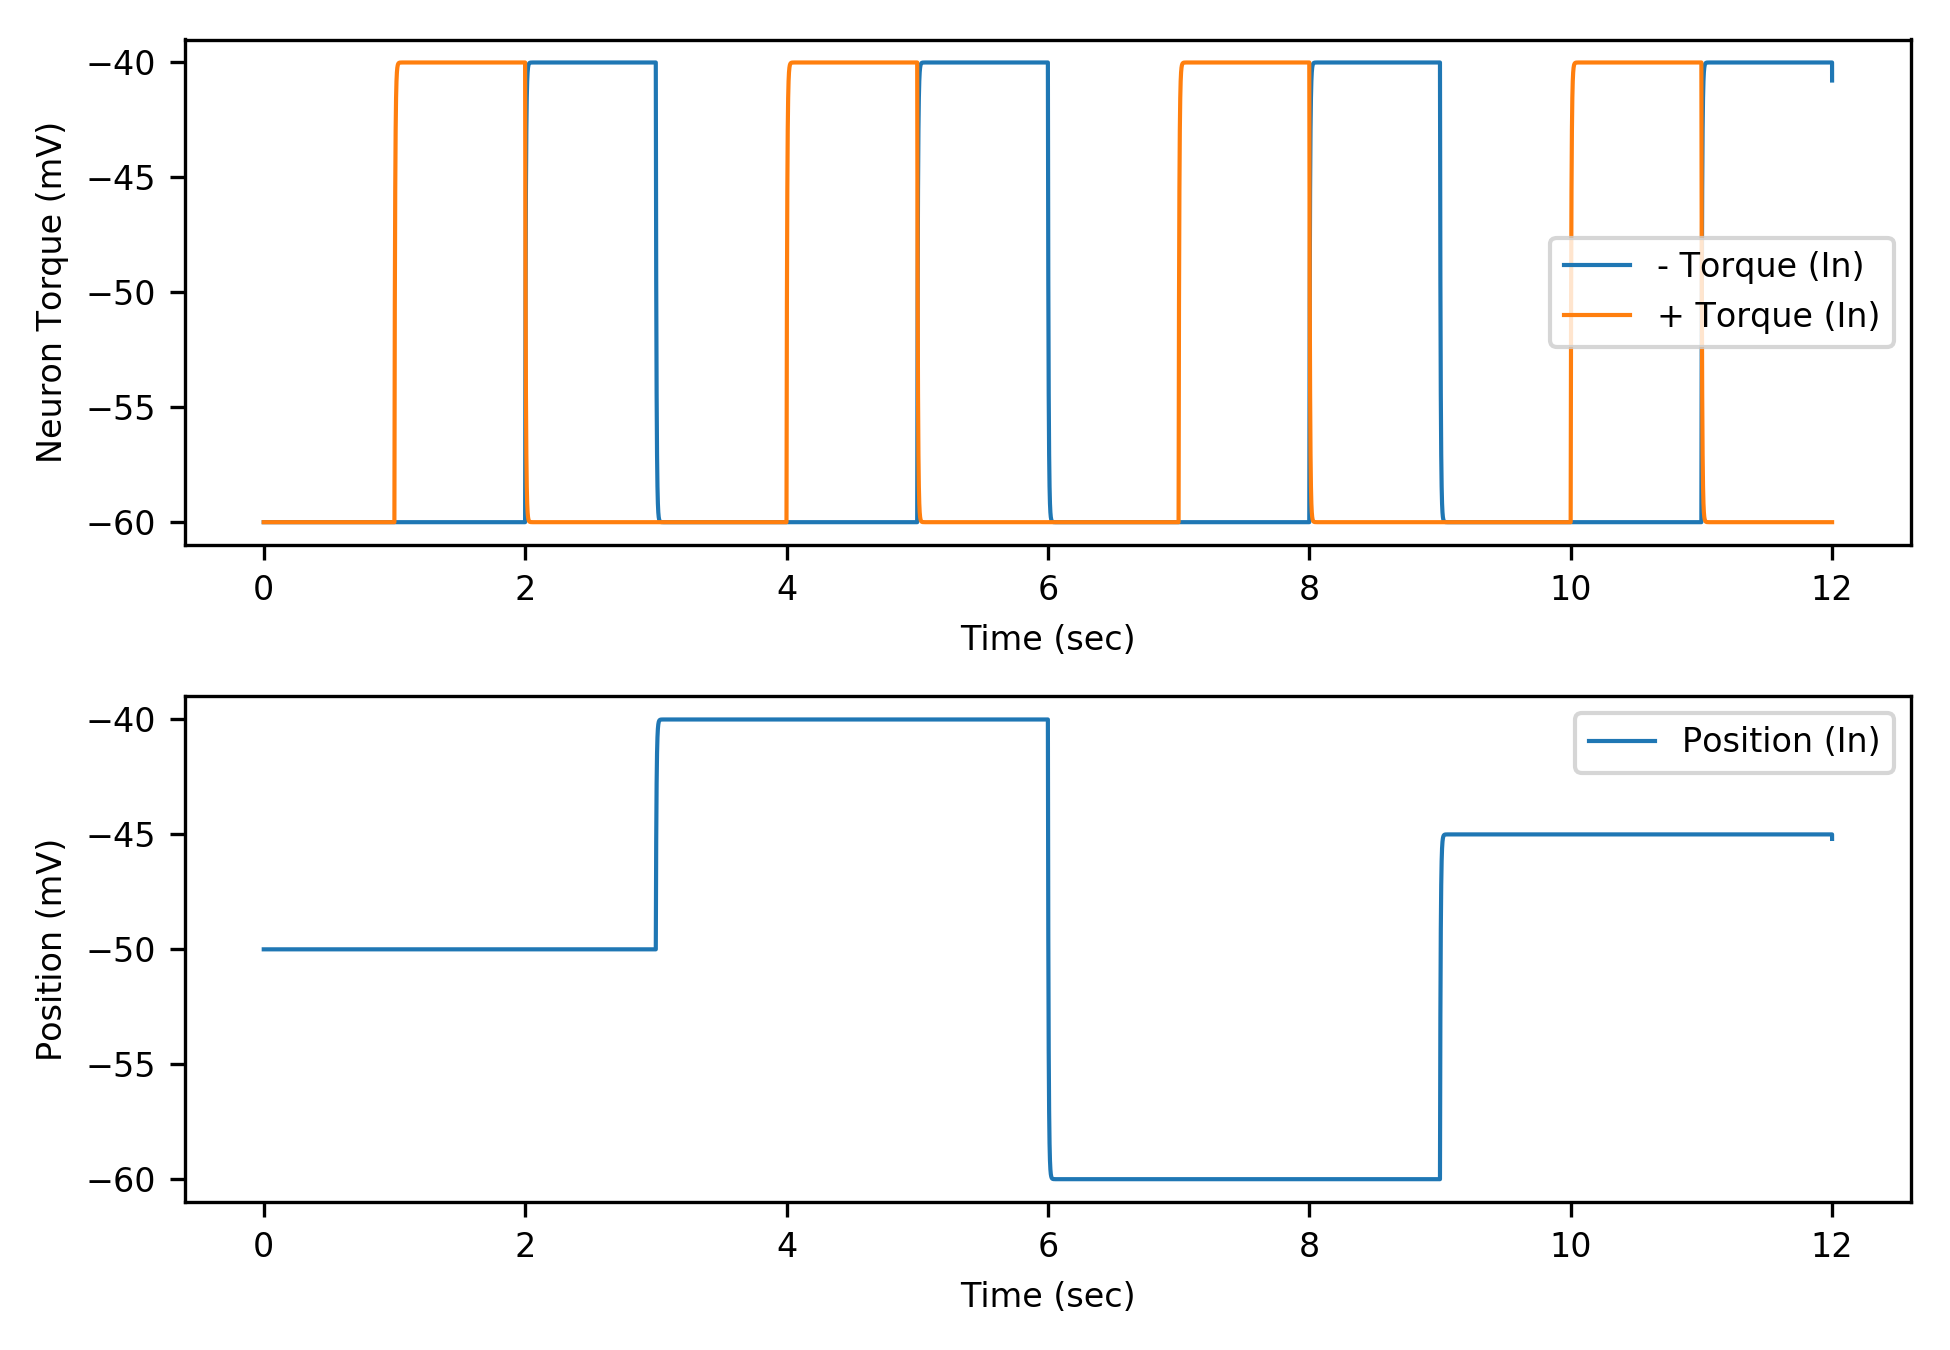
\includegraphics[height=3.5in]{methods/T2PInput}
\caption{Drive inputs to test the pressure network}
\label{fig:TestNetworkInputs}
\end{figure}

The test frameworks can be rigged at multiple levels to enable testing of
individual units and the integration of units in the style of unit tests and
integration tests from a more traditional software background.
